\documentclass[nooutcomes]{ximera}
%% handout
%% space
%% newpage
%% numbers
%% nooutcomes


\newcommand{\RR}{\mathbb R}
\renewcommand{\d}{\,d}
\newcommand{\dd}[2][]{\frac{d #1}{d #2}}
\renewcommand{\l}{\ell}
\newcommand{\ddx}{\frac{d}{dx}}
\newcommand{\dfn}{\textbf}
\newcommand{\eval}[1]{\bigg[ #1 \bigg]}

\usepackage{multicol}

\renewenvironment{freeResponse}{
\ifhandout\setbox0\vbox\bgroup\else
\begin{trivlist}\item[\hskip \labelsep\bfseries Solution:\hspace{2ex}]
\fi}
{\ifhandout\egroup\else
\end{trivlist}
\fi} %% we can turn off input when making a master document

\usepackage{fullpage}


\title{Recitation \ 2.1:  The Idea of Limits}  

\begin{document}
\begin{abstract}		\end{abstract}
\maketitle


%problem 1
 \begin{problem} What does the secant line to a linear function look like?  What does a tangent line to a linear function look like? 
  	 \begin{freeResponse}		 
	Both the secant and tangent lines are the linear function itself.
	\begin{image}
	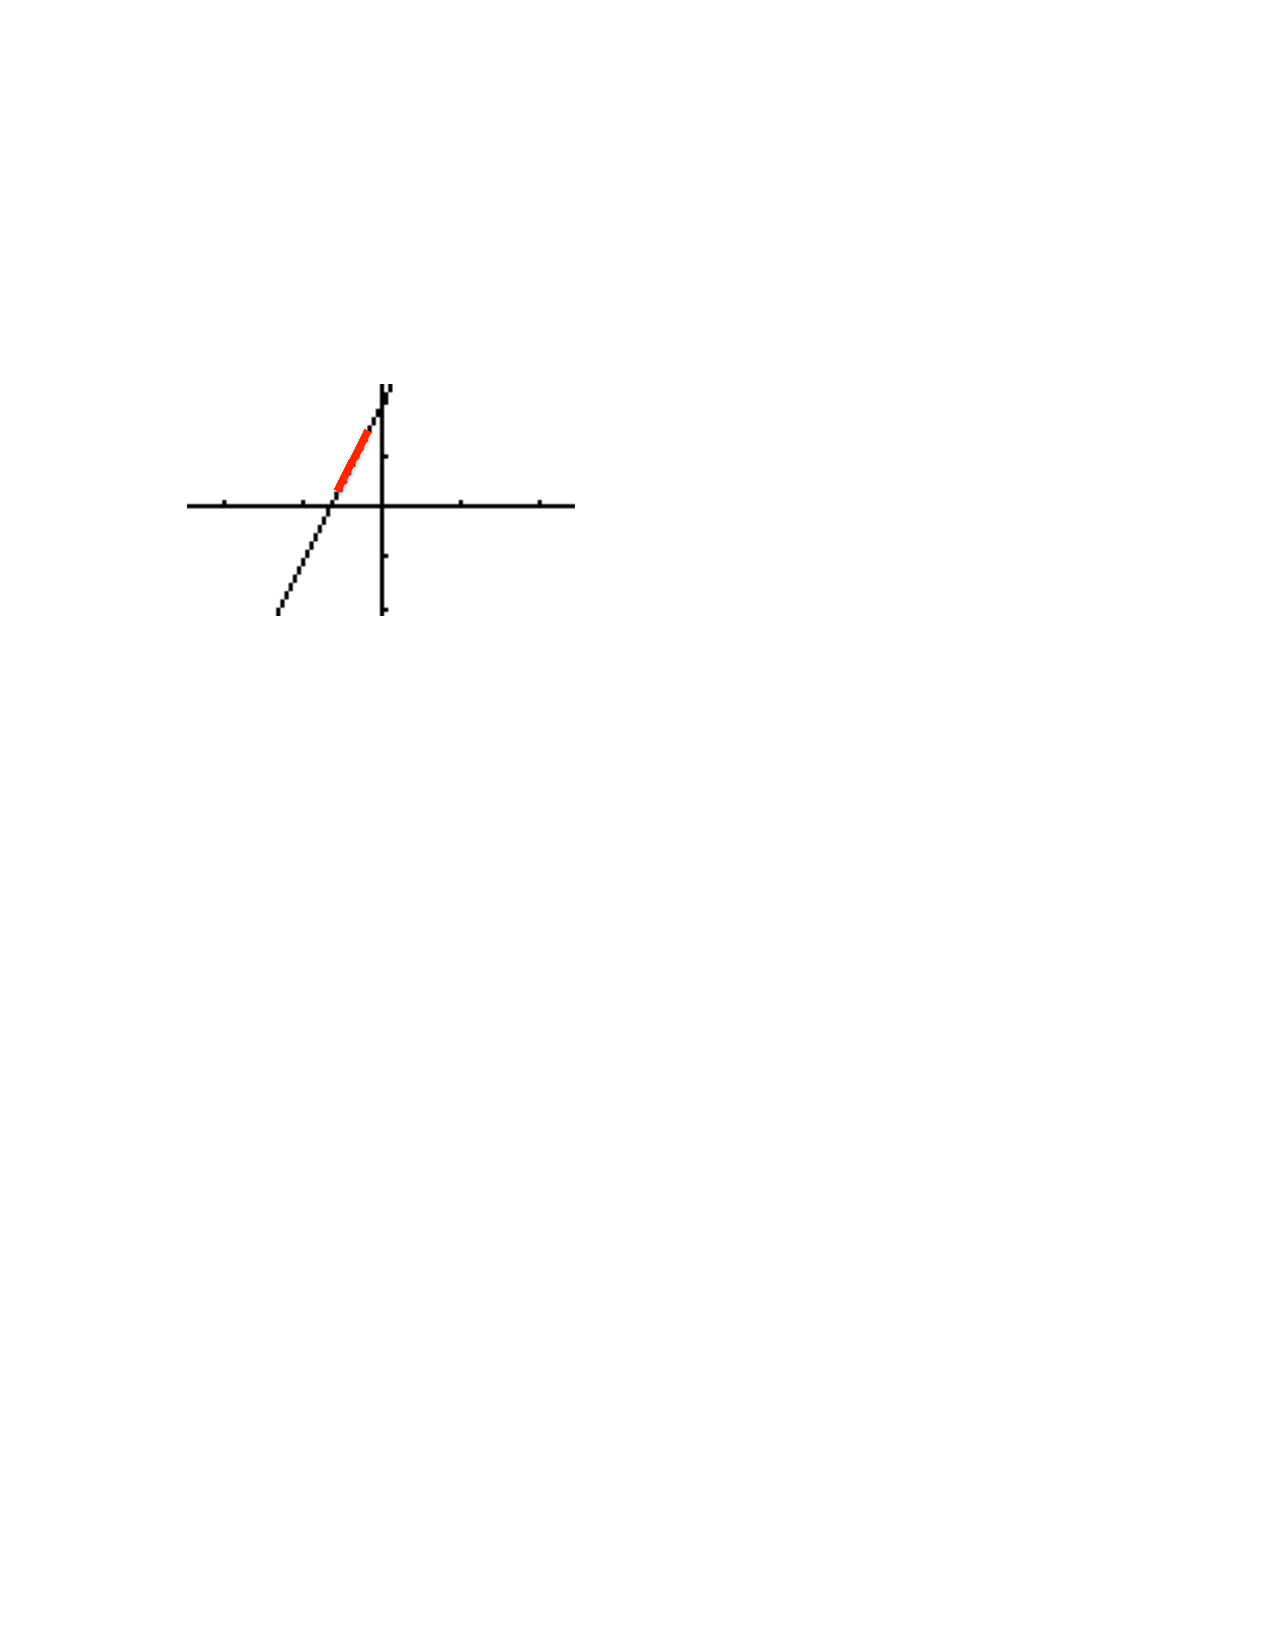
\includegraphics[trim= 90 480 300 160]{Figure8.pdf}
	\end{image}
	\end{freeResponse}


\begin{problem}
Below is a graph and two tables of values of the height (in feet) of a ball thrown straight up into the air.   The height of the ball $x$ seconds after being released is given by the function $f(x)=-16x^2+128x+144$.  The viewing window is [-5,10] x [-100,500].
	
	
	
	
\[ \begin{array}{lr}

\small{	
\begin{tabular}{|l|l|}
\hline
\hspace{2mm} $x$ & \hspace{4mm} $f(x)$  \\
\hline
2 & 336  \\
\hline
2.0001 & 336.00639...  \\
\hline
2.001 & 336.06398....  \\
\hline
2.01 & 336.634  \\
\hline
2.1 & 342.24  \\
\hline
... & ...  \\
\hline
8.9 & 15.84  \\
\hline
8.99 & 1.5984  \\
\hline
8.999 & 0.159984  \\
\hline
8.9999 & 0.0159998...  \\
\hline
9 & 0 \\
\hline
\end{tabular}
}

&  

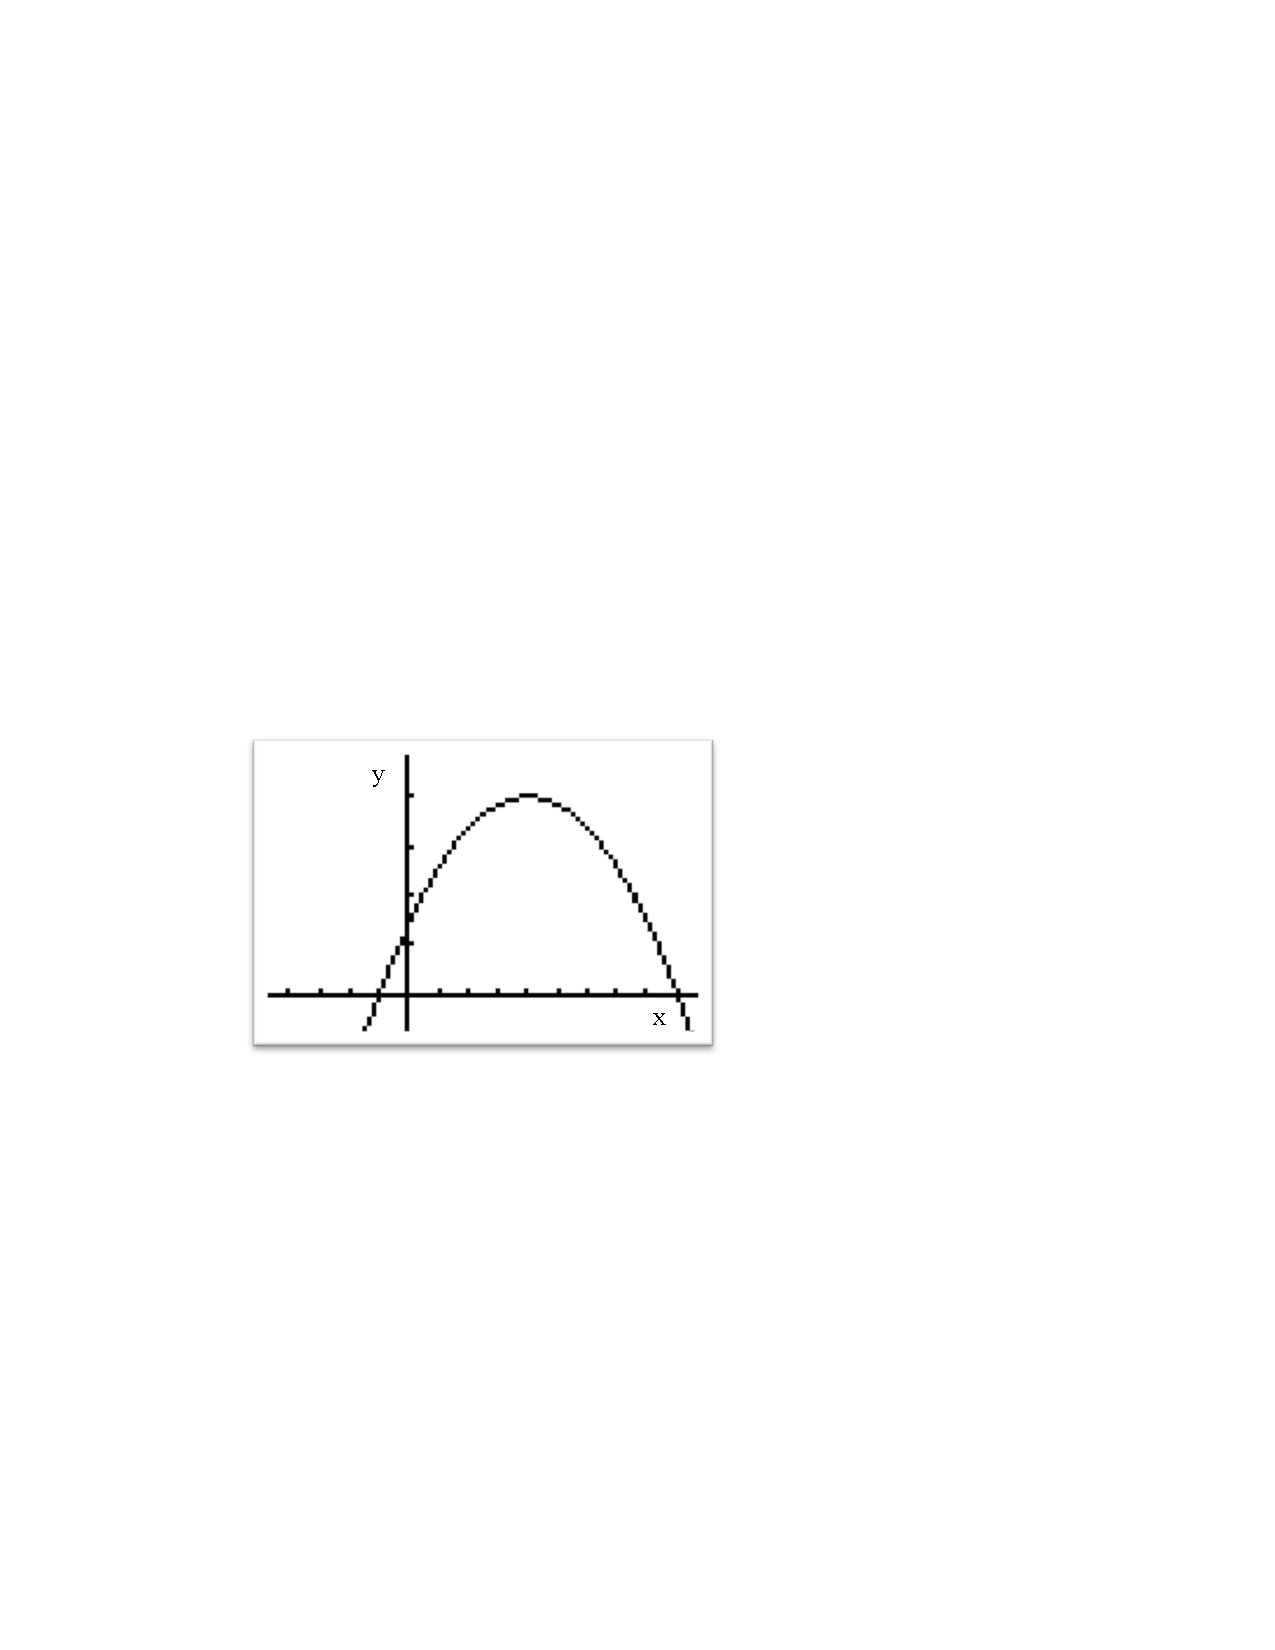
\includegraphics[trim= 100 360 300 350]{Figure9.pdf}


\end{array} \]



	
		\begin{enumerate}
			
		 \item  What are the units on the $x$ and $y$ axis?
		 \begin{freeResponse}		 
		The units on the $x$-axis are seconds (time), the units on the $y$-axis are feet (height).
		\end{freeResponse}
			
		\item  Is the graph a picture of the path that the ball follows?  Why or why not?
		\begin{freeResponse}		 
		 The graph is not a picture of the path the ball follows.  The graph shows the height of the ball at a given \emph{time}.  The ball is thrown straight up and has no horizontal movement.
		\end{freeResponse}
	
		\item  When will the ball hit the ground?
		\begin{freeResponse}		 
		The ball will hit the ground when the height $f(x)$ equals zero.
			\begin{align*}
			0&=-16t^2+128t+144 \\
			0&=-16(t^2-8t-9) \\
 			0&=-16(t+1)(t-9) \\
 			t&=-1,9 
 			\end{align*}
		\end{freeResponse}
		
		
	
		\item  Make a table of average velocities and use it to approximate the instantaneous velocity of the ball when it hits the ground.
		\begin{freeResponse}		 
			\begin{tabular}{|l|l|}
			\hline
			\text{Time Interval} & \text{Average Velocity}  \\
			\hline
			[8.9, 9] & $\frac{f(9)-f(8.9)}{.1}=\frac{0-15.84}{.1}=-158.4$  \\
			\hline
			[8.99,9] & $\frac{f(9)-f(8.99)}{.01}=\frac{0-1.5984}{.01}=-159.84$  \\
			\hline
			[8.999, 9] & $\frac{f(9)-f(8.999)}{.001}=\frac{0-.159984}{.001}=-159.984$  \\
			\hline
			[8.9999, 9] &  $\frac{f(9)-f(8.999)}{.0001}=\frac{0-.0159998}{.0001}=-159.998$  \\
			\hline
			\end{tabular}
		\end{freeResponse}
		
		
			
		\item  Using the graph, determine at what times does the ball have an instantaneous velocity of zero.  How do you know?
		\begin{freeResponse}		 
		At time $t$ equals about 4 seconds, the ball has an instantaneous velocity of zero because it looks like the slope of the tangent line to the curve at time $t$ equals 4 is zero (The tangent line is a horizontal line).
			\begin{image}
			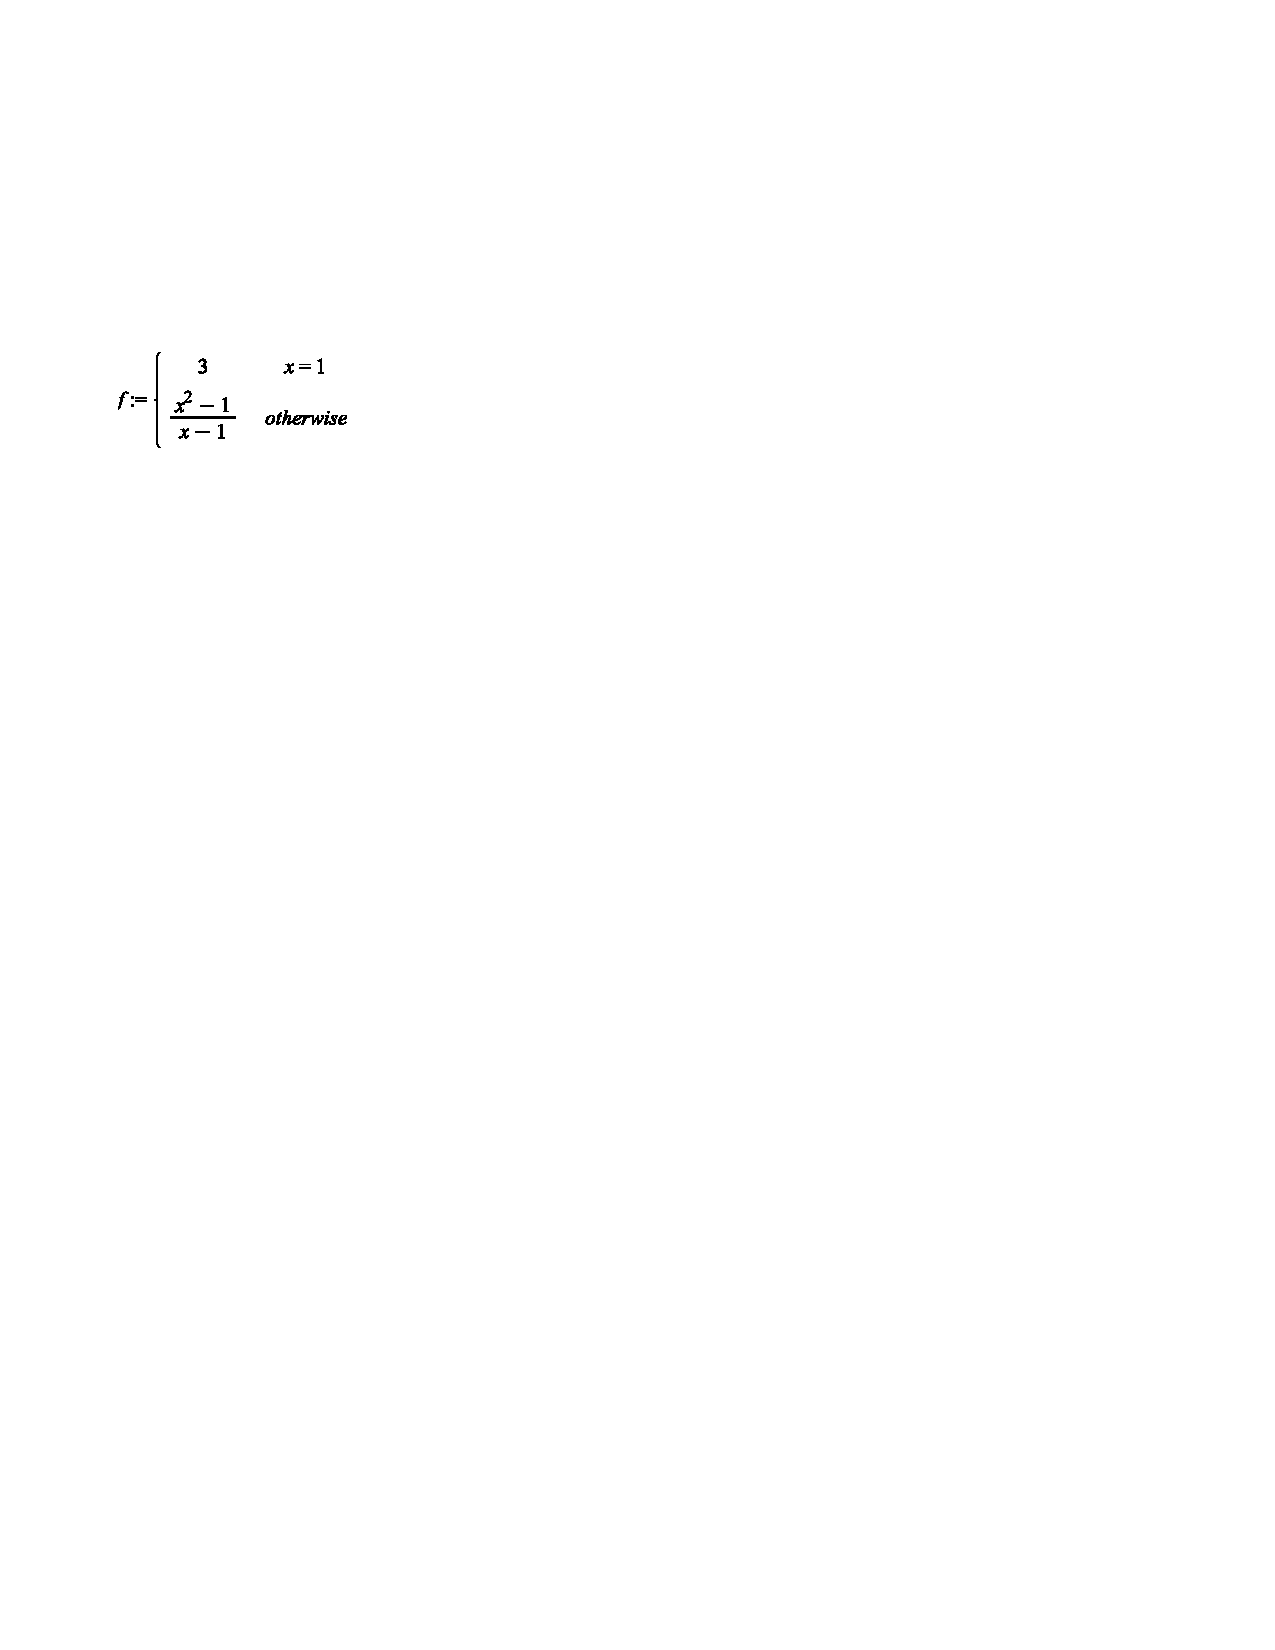
\includegraphics[trim= 80 470 300 180]{Figure7.pdf}
			\end{image}
		\end{freeResponse}
		
		
		
		\item  For what times is the instantaneous velocity negative?  What is happening to the height of the ball at those times?
			
		\begin{freeResponse}		 
		The instantaneous velocity is negative at all times after 4 seconds.  We know this because the graph is ``moving downwards'' (which is equivalent to all tangent lines having negative slope).  The height of the ball is decreasing at those times because the direction of the velocity is downward (negative) and as we move forward in time, the $y$-values (or height values) are decreasing. 
		\end{freeResponse}
			
		\end{enumerate}
			
\end{problem}
			
			
			
			
			
\begin{problem}
Consider the function$f(x)=x^2+2x$.  A table of values and graph for this function $f(x)$ are given below.

\[ \begin{array}{lr}

\small{			
\begin{tabular}{|l|l|}
\hline
\hspace{2mm} $x$ & \hspace{4mm} $f(x)$  \\
\hline
1.9 & 7.41  \\
\hline
1.95 & 7.7025  \\
\hline
1.99 & 7.9401  \\
\hline
1.999 & 7.994001  \\
\hline
1.9999 & 7.99940001  \\
\hline
2 & 8  \\
\hline
2.0001 & 8.00060001  \\
\hline
2.001 & 8.006001  \\
\hline
2.01 & 8.0601  \\
\hline
2.05 & 8.3025  \\
\hline
2.1 & 8.61 \\
\hline
\end{tabular}
}

& 

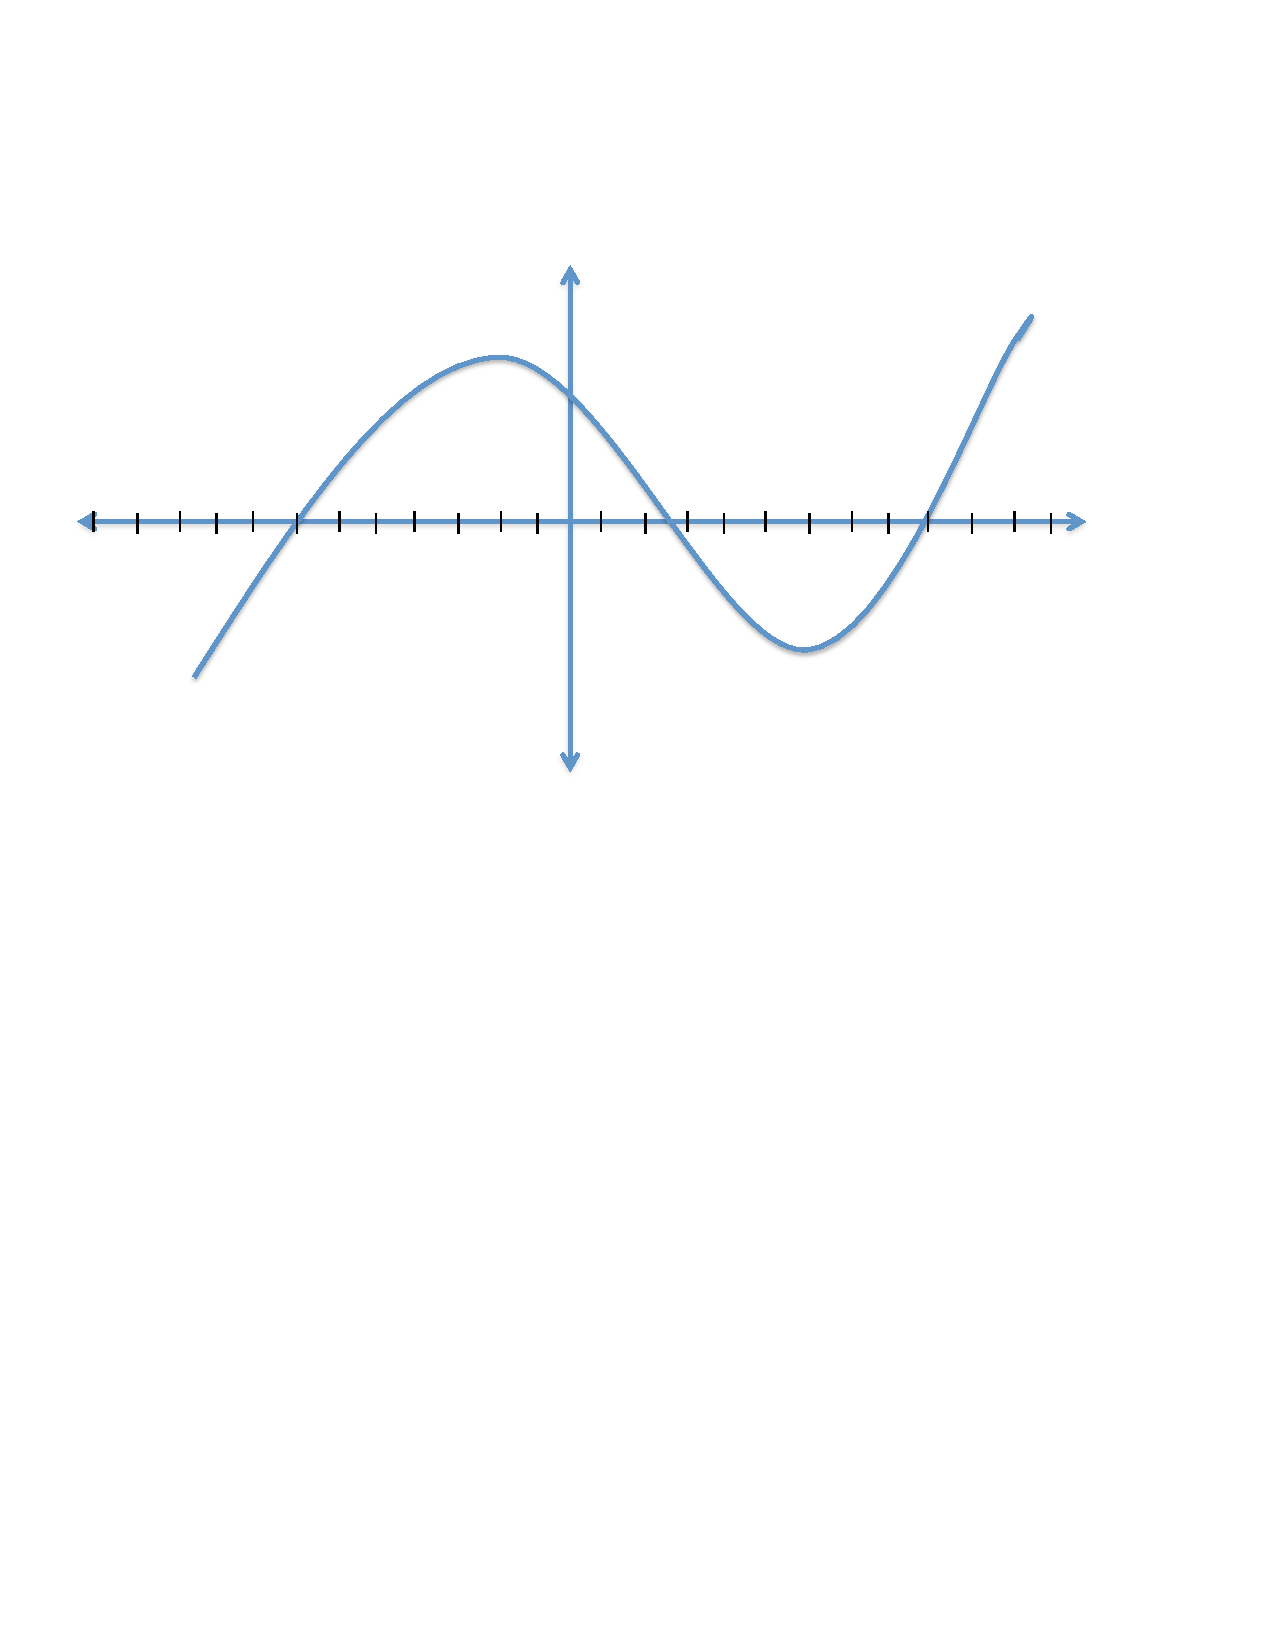
\includegraphics[trim= 250 560 150 250]{Figure2.pdf} 

\\

\end{array} \]
	
		\begin{enumerate}
			
		\item  Make a table of slopes of secant lines between $x=2$ and $x=a$ where $a$ approaches 2.  Then approximate the slope of the tangent line at the point $x=2$.
		\begin{freeResponse}		 
		We need to find secant lines around the point $x=2$.
		
			\begin{tabular}{|l|l|}
			\hline
			Interval & Slope of Secant Line  \\
			\hline
			[1.9,2] & $ \frac{f(2)-f(1.9)}{.1}=\frac{8-7.41}{.1}=5.9$  \\
			\hline
			[1.99,2] & $\frac{f(2)-f(1.99)}{.01}=\frac{8-7.9401}{.01}=5.99$  \\
			\hline
			[1.999,2] & $\frac{f(2)-f(1.999)}{.001}=\frac{8-7.994001}{.001}=5.999$  \\
			\hline
			[1.9999,2] & $\frac{f(2)-f(1.9999)}{.0001}=\frac{8-7.99940001}{.0001}=5.9999$  \\
			\hline
			\end{tabular}
			
			\begin{tabular}{|l|l|}
			\hline
			Interval & Slope of Secant Line  \\
			\hline
			[2,2.1] & $ \frac{f(2.1)-f(2)}{.1}=\frac{8.61-8}{.1}=6.1$  \\
			\hline
			[2,2.01] & $\frac{f(2.01)-f(2)}{.01}=\frac{8.0601-8}{.01}=6.01$  \\
			\hline
			[2,2.001] & $\frac{f(2.001)-f(2)}{.001}=\frac{8.006001-8}{.001}=6.001$  \\
			\hline
			[2,2.0001] & $\frac{f(2.0001)-f(2)}{.0001}=\frac{8.00060001-8}{.0001}=6.0001$  \\
			\hline
			\end{tabular}
			
		The approximate slope of the tangent line at $x=2$ is 6.
		\end{freeResponse}
			  
		\item  Draw a secant line on the interval $[1,3]$ onto the graph of the function.  Then draw the tangent line at $x=2$ onto the graph. 
		\begin{freeResponse}		 
		The secant line is purple, and the tangent line is red (imagine that the red line just touches the curve at $x=2$, it is really close!).
			\begin{image}
			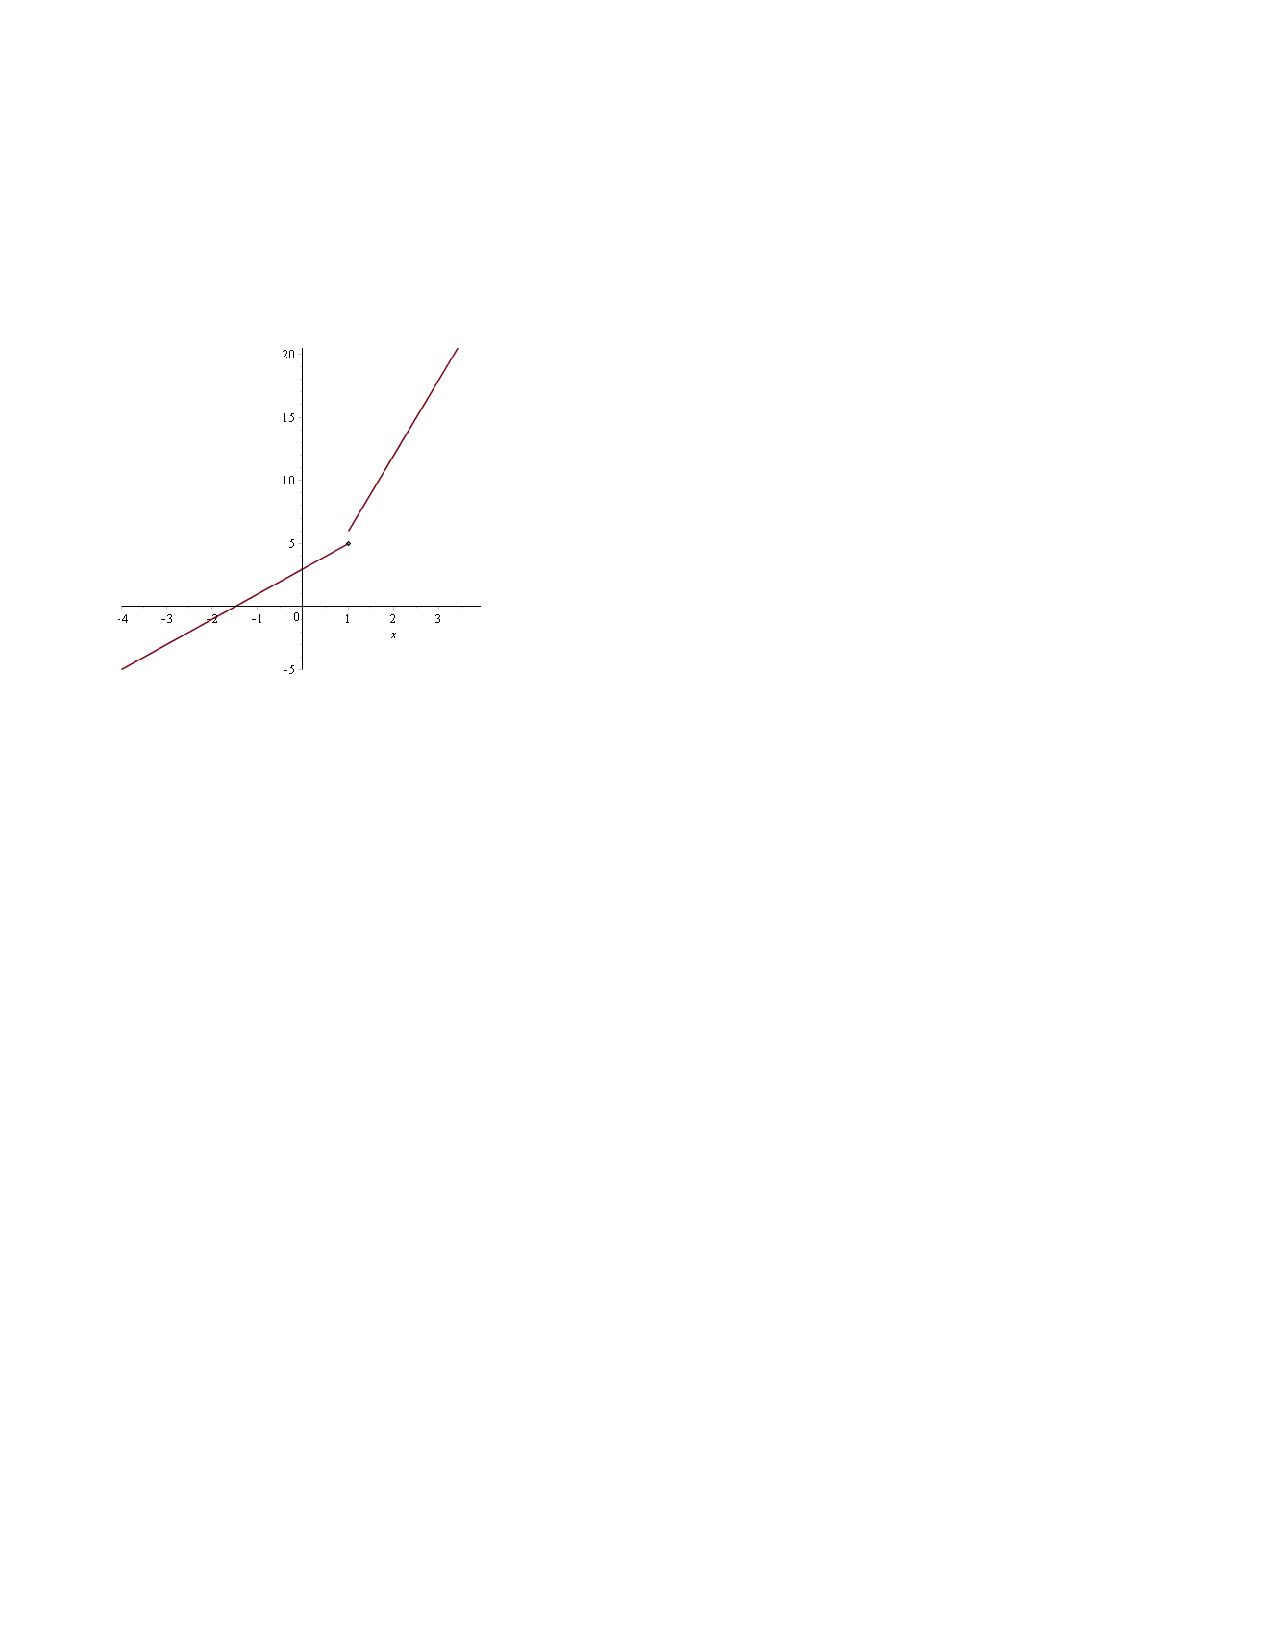
\includegraphics[trim= 80 500 300 160]{Figure6.pdf}
			\end{image}
		\end{freeResponse}
				
		\end{enumerate}
			
			
			

	
\end{problem}










								
				
\end{document} 


















